Aufgrund der hohen Popularität der $\lambda$-Architektur, gibt es Dienste, die sowohl Echtzeitverarbeitung, als auch Batch/\ac{OLAP}-Verarbeitung unterstützen.

\subsection{AWS IoT Analytics} \label{productselection:iotanalytics}



\AWSIOT{} Analytics ist ein Dienst der \AWSIOT{} Familie, der nach Aussage des Herstellers weitreichende Analysen von \ac{IoT} Daten, die beispielsweise via \AWSIOT{} Core geladen werden können, zulässt.\footcite[Vgl. auch im Folgenden][]{AmazonWebServicesInc..o.J.c} Dabei bietet der Dienst Lösungen für Sammlung, Verarbeitung, Speicherung, Analyse und Benachrichtigung/Visualisierung von Daten an, bzw. bietet Schnittstellen, um diese Aufgaben zu erledigen. Im speziellen deckt \AWSIOT{} Analytics die Aufgaben einer $\lambda$-Architektur ab. So besitzt \AWSIOT{} Analytics beispielsweise eine integrierte Zeitreihendatenbank, welche ergänzend zu den Echtzeitdaten von \AWSIOT{} Core für Analysen genutzt werden kann.
\begin{figure}[H]
\centering
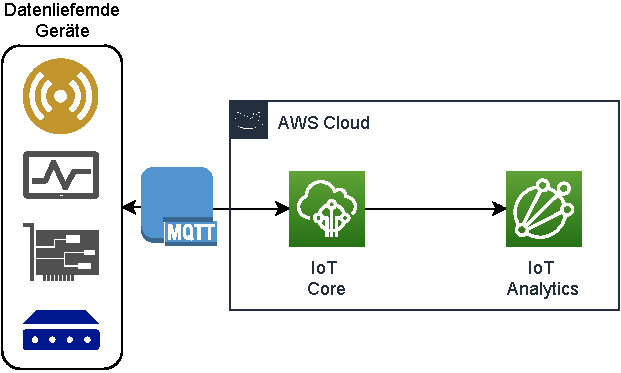
\includegraphics[width=0.8\textwidth]{graphics/IoT-Analytics-general.pdf}
\caption{Grobarchitektur des Ablaufes für IoT Analytics}
\label{abb:GrobArchitekturIoTAnalytics}
\end{figure}
In \autoref{abb:GrobArchitekturIoTAnalytics} ist die Grobarchitektur und Verknüpfung mit anderen Diensten unter Annahme der Vorraussetzungen aus \autoref{chap:rahmendatenverarbeitung} gezeigt. Datenliefernde Geräte, wie beispielsweise Sensoren, liefern Zeitreihen-Messwerte via dem \ac{MQTT} Protokoll an. Die Weiterleitung zu IoT Analytics erfolgt mittels einer eingerichteten Regel im \ac{IoT} Core Messagebroker, welche mittels eines Dialekts der \ac{SQL} Sprache gewisse Topics vorselektiert oder alle Topics zulässt.


Für erweiterte Analysen stellt \AWSIOT{} Analytics sogenannte Notebooks zur Verfügung, die auf den \enquote{Jupyter Notebooks} basieren. Diese Notebooks werden verwendet, um Python Programmabläufe zu visualieieren und zu modularisieren. Da in den Jupyter Notebooks der volle Paketumfang von Python verfügbar ist, inklusive z.B. Machine Learning Bibliotheken wie Tensorflow, sind wesentlich erweiterte Analysen möglich. Die Ressourcen für Notebooks sind seperat zu provisionieren und werden in Analytics Compute Units abgerechnet, wobei eine Compute Unit 4vCPU-Kerne und 16 GB \ac{RAM} hat.\footcite[Vgl.][]{AmazonWebServicesInc..o.J.i} Diese Compute Units werden sekundengenau abgerechnet und kosten nur für die Laufzeit Geld.

\subsubsection{Gesamtkosten}
In \autoref{tab:kostenvergleich-AWS~IoT~Analytics} sind die kalkulierten Preise nach gängiger Preismatrix dargestellt.\footcite[Vgl. auch im Folgenden][]{AmazonWebServicesInc..o.J.i} Die Nutzung von externen Ausführungsdiensten (z.B. StepFunctions/Lambda) für \ac{SQL}-Abfragen ist nicht notwendig, da die Abfragen im Dienst selbst terminiert werden können.
\begin{table}[H]
\centering
\begin{tabular}{|l|l|l|}
\hline
Dimension & Preis(\$)/Einheit & Summe (\$) \\ \hline
Datenspeicherung (roh+verarbeitet)  & \begin{tabular}[c]{@{}l@{}}0,03/GB (verarbeitet) \\ 0,023 (roh)\end{tabular} & 7,77  \\\hline
Anfragenbearbeitung & \begin{tabular}[c]{@{}l@{}}0,00634/GB\end{tabular} & 121,50 \\ \hline
\begin{tabular}[c]{@{}l@{}}Eigene Analyselogik \\ 960 Abfragen * 5 Sekunden\end{tabular}  & 0,36/h & 0,48  \\\hline
Summe & \cellcolor[HTML]{EFEFEF} & \underline{129,75}  \\\hline

\end{tabular}
\caption{Kostenvergleich AWS~IoT~Analytics}
\label{tab:kostenvergleich-AWS~IoT~Analytics}
\end{table}
 Das bestehende \enquote{Free Tier}, welches \ac{AWS} für den Dienst anbietet, wird ignoriert, da es nur in den ersten zwölf Monaten der Nutzung des Dienstes verrechnet wird. Bei \ac{S3} wird angenommen, dass die Standard Speicherklasse verwendet wird und Volumenrabattierungen bei Datenvolumina >50TB im Monat nicht relevant sind.\footcite[Vgl. auch im Folgenden][]{AmazonWebServicesInc..o.J.j} Andere Speicherklassen sind günstiger, somit gibt die Schätzung eine Obergrenze für die \ac{S3} Preise. Es wurde ebenfalls keine eigene Logik in Notebooks kalkuliert, welche 0,36\$ pro Stunde und Compute Unit im Betrieb kosten würden. Dies ist dem Fakt geschuldet, dass für dieses Beispiel die Analysen mit \ac{SQL} bewältigbar sind.
 
\subsubsection{Weitere Evaluationen}
Die Performance und Verfügbarkeit sowie die Features werden in \anhangref{anhang:vergleich-iot-analytics} diskutiert.

\subsection{Auswahl}
Im Bereich Multimode gibt es nur einen zu vergleichenden Dienst, weshalb Abzüge nicht auf relativen Kriterien zu den anderen Diensten basieren, sondern auf absoluten Abzügen.
\begin{table}[H]
    \centering
    \begin{tabular}{|l|l!{\vrule width 2pt}l|}
    \hline
\multicolumn{1}{|c|}{Kriterium} & \multicolumn{1}{c!{\vrule width 2pt}}{\begin{tabular}[c]{@{}c@{}}max.\\Punkte\end{tabular}} & \multicolumn{1}{c|}{\begin{tabular}[c]{@{}c@{}}AWS\\IoT\\Analytics\end{tabular}} \\ \hline
     \begin{tabular}[c]{@{}l@{}}Übertragbarkeit zwischen \\ Clouds (ISO 9126)\end{tabular} & 1 & 0 \\ \hline
     \begin{tabular}[c]{@{}l@{}}Integration mit anderen \\ \ac{AWS} Diensleistungen\end{tabular} & 3 & 3 \\ \hline
     Generalisierung & 4 & 3 \\ \hline
     Erweiterbarkeit & 4 & 4 \\ \hline
     \begin{tabular}[c]{@{}l@{}}Fehlertransparenz/ \\ \textit{Debugability}\end{tabular} & 5 & 4 \\ \hline
     \begin{tabular}[c]{@{}l@{}}geringer \\ Wartungsaufwand\end{tabular} & 7 & 4 \\ \hline
     \begin{tabular}[c]{@{}l@{}}Skalierbarkeit \& \\ \textit{serverlessness}\end{tabular} & 7 & 6 \\ \hline
     Kosten & 7 & 5 \\ \hline
     Performancegarantien & 8 & 7 \\ \hline
     \begin{tabular}[c]{@{}l@{}}Robustheit \& \\ Fehlertoleranz\end{tabular} & 9 & 7 \\ \hline
     \begin{tabular}[c]{@{}l@{}}Auswertungen \\ (\autoref{chap:auswertungsarten}) \end{tabular} & 11 & 11 \\ \hlinewd{2pt}
     \rowcolor[HTML]{ECF4FF}
     Summe & 66 & \textbf{\cellcolor[HTML]{ECF4FF}54} \\ \hline
\end{tabular}
\caption{Bewertungsmatrix~Multimode}
\label{tab:bewertungsmatrix-multimode}
\end{table}
Klar ist, dass zwar bei \AWSIOT{} Analytics die Jupyter Notebooks plattformunabhängig sind, aber die \ac{SQL}-Statements nicht übertragbar sind und zwingend ein \AWSIOT{} Core Broker benötigt wird. Aufgrund dieses \textit{vendor-lockins} kann ein großer Teil des Setups nicht übertragen werden.
\AWSIOT{} Analytics integriert sich gut mit anderen Dienstleistungen von AWS, z.B. mit \AWSIOT{} Core und den anderen \AWSIOT{} Diensten, SageMaker, QuickSight , Lambda, \ac{SNS} und weiteren.
\AWSIOT{} Analytics ist speziell für \ac{IoT} Daten gebaut, weshalb Funktionalitäten eingebaut sind, die speziell in Kombination mit den anderen \AWSIOT{} Diensten Sinn machen. Die Verwendung dieser Funktionalitäten ist aber nicht zwingend notwendig. Es können auch andere Daten, z.B. IT-Monitoring eingespeist werden, wenn sie über \ac{MQTT} und den \AWSIOT{} Core Broker geladen werden.
Die Erweiterbarkeit ist gegeben durch die Möglichkeiten, die \ac{SQL} in Verbindung mit der generischen Programmierbarkeit der Notebooks bietet und zusätzlich dadurch, dass durch die integrierte Datenbank Daten erneut mit anderer Logik verarbeitet werden können.
Durch Integration mit Cloudwatch, der Monitoring Lösung von \ac{AWS} sind ansteigende Fehlerraten leicht zu entdecken. Einzig, dass eingehende Daten einige Zeit benötigen, bis sie von der \AWSIOT{} Analytics Konsole angezeigt werden, kann die Fehlersuche erschweren.\footcite[Vgl.][]{AmazonWebServicesInc..o.J.aw}
Im Bereich \enquote{serverlessness} wurden Abzüge getätigt, da Analyitcs Compute Units nicht selbstständig skalieren.
Da die Abfragekosten mittels \ac{SQL} proportional zu den anderen Kosten hoch erscheinen, wurden Abzüge gemacht.
Die gesetzten Performancelimits des Dienstes erscheinen sinnvoll. Eine Fehlertoleranz ist gegeben, wenn der Anwender keine Fehler selbst einführt, oder \AWSIOT{} Analytics interne Fehler aufweist. Da alle Auswertungen sogar in multiplen Wegen machbar sind, wurde die volle Punktzahl für diese Kategorie vergeben. Im Vergleich zu den spezialisierteren Diensten, die dem $kappa$ oder \ac{OLAP} Muster folgen, schneidet \AWSIOT{} Analytics schlechter ab. Dies ist bedingt durch die wesentlich höheren monatlichen Kosten, genauso wie durch eine fehlende Garantie der schnellen Datenverarbeitung, zu welcher Kinesis fähig ist. Das $lambda$ Pattern scheint in dieser Implementierung ein nachteiliger Kompromiss aus der Kombination von $kappa$ und \ac{OLAP} zu sein.

\subsubsection{Übertragbarkeit zwischen Clouds}
\subsubsection{Integration mit AWS}
\subsubsection{Generalisierung}
\subsubsection{Erweiterbarkeit}
\subsubsection{Fehlertransparenz}
\subsubsection{geringer Wartungsaufwand}
\subsubsection{Skalierbarkeit \& serverlessness}
\subsubsection{Kosten}
\subsubsection{Performancegarantien}
\subsubsection{Robustheit \& Fehlertoleranz}
\subsubsection{Auswertungen}
\subsubsection{Summe}
